\documentclass[letterpaper,11pt,oneside,reqno]{article}

%%%%%%%%%%%%%%%%%%%%%%%%%%%%%%%%%%%%%%%%%%%%%%%%%%%%%%%%%%%%

\usepackage[pdftex,backref=page,colorlinks=true,linkcolor=blue,citecolor=red]{hyperref}
\usepackage[alphabetic,nobysame]{amsrefs}

%%%%%%%%%%%%%%%%%%%%%%%%%%%%%%%%%%%%%%%%%%%%%%%%%%%%%%%%%%%%
%main packages
\usepackage{amsmath,amssymb,amsthm,amsfonts,mathtools}
\usepackage{graphicx,color}
\usepackage{upgreek}
\usepackage[mathscr]{euscript}

%equations
\allowdisplaybreaks
\numberwithin{equation}{section}

%tikz
\usepackage{tikz}
\usetikzlibrary{shapes,arrows,positioning,decorations.markings}

%conveniences
\usepackage{array}
\usepackage{adjustbox}
\usepackage{cleveref}
\usepackage{enumerate}
\usepackage{datetime}

%paper geometry
\usepackage[DIV=12]{typearea}

%%%%%%%%%%%%%%%%%%%%%%%%%%%%%%%%%%%%%%%%%%%%%%%%%%%%%%%%%%%%
%draft-specific
\synctex=1
% \usepackage{refcheck,comment}

%%%%%%%%%%%%%%%%%%%%%%%%%%%%%%%%%%%%%%%%%%%%%%%%%%%%%%%%%%%%
%this paper specific
\newcommand{\ssp}{\hspace{1pt}}

%%%%%%%%%%%%%%%%%%%%%%%%%%%%%%%%%%%%%%%%%%%%%%%%%%%%%%%%%%%%
\newtheorem{proposition}{Proposition}[section]
\newtheorem{lemma}[proposition]{Lemma}
\newtheorem{corollary}[proposition]{Corollary}
\newtheorem{theorem}[proposition]{Theorem}
%%%%%%%%%%%%%%%%%%%%%%%%%%%%%%%%%%%%%%%%%%%%%%%%%%%%%%%%%%%%
\theoremstyle{definition}
\newtheorem{definition}[proposition]{Definition}
\newtheorem{remark}[proposition]{Remark}
%%%%%%%%%%%%%%%%%%%%%%%%%%%%%%%%%%%%%%%%%%%%%%%%%%%%%%%%%%%%

\begin{document}
\title{Lectures on Random Matrices
(Spring 2025)
\\Lecture 7: Double contour integral kernel. Steepest descent and local statistics}


\date{Monday, February 24, 2025\footnote{\href{https://lpetrov.cc/rmt25/}{\texttt{Course webpage}}
$\bullet$ \href{https://lpetrov.cc/simulations/model/random-matrices/}{\texttt{Live simulations}}
$\bullet$ \href{https://lpetrov.cc/rmt25/rmt25-notes/rmt2025-l07.tex}{\texttt{TeX Source}}
$\bullet$
Updated at \currenttime, \today}}



\author{Leonid Petrov}


\maketitle
\tableofcontents


\section{Steepest descent for the GUE kernel}
\label{sec:steepest-descent-GUE}

\subsection{Scaling}
\label{sub:scaling}

Let us now consider the GUE kernel
\eqref{eq:K_n_conjugated},
\begin{equation*}
	K_n(x,y)=\frac{1}{(2\pi)^2}
	\oint_C dt\int_{-i\infty}^{i\infty}ds\ssp
	\frac{\exp\left\{ \frac{s^2}{2}-sy-\frac{t^2}{2}+tx \right\}}{s-t}\left( \frac{s}{t} \right)^n
	,
\end{equation*}
where the integration contours are as in \Cref{fig:contours}.

We know from the Wigner semicircle law
(established for real symmetric matrices with general iid entries in
in \href{https://lpetrov.cc/rmt25/rmt25-notes/rmt2025-l02.pdf}{Lecture 2},
and for the GUE in \href{https://lpetrov.cc/rmt25/rmt25-notes/rmt2025-l04.pdf}{Lecture 4})
that the eigenvalues live on the scare $\sqrt n$. This means that to capture the local asymptotics,
we need to scale
\begin{equation}
	\label{eq:scaling_x-y}
	x=X\sqrt n+\frac{\Delta x}{\sqrt n},\qquad y=Y\sqrt n+\frac{\Delta y}{\sqrt n},\qquad
	\Delta x,\Delta y\in\mathbb{R}.
\end{equation}
Moreover, if $X\ne Y$ (i.e., different global positions), one can check that the kernel
vanishes. In other words, the local behaviors at different global positions are independent.
See Problem~\ref{prob:different-global-positions}.
In what follows, we take $Y=X$.

Let us also make a change of the integration variables:
\begin{equation*}
	t=z\sqrt n,\qquad s=w\sqrt n.
\end{equation*}
The integration contours for $z$ and $w$ look the same as in
\Cref{fig:contours}, up to a rescaling. However, as $0$
and $t=s$
are the only singularities in the integrand, we can deform the $z,w$
contours as we wish, while keeping $|z|<|w|$
and the general shape as in \Cref{fig:contours}.

We thus have:
\begin{multline}
	\label{eq:K_n_scaling}
	K_n(X\sqrt n+\Delta x/\sqrt n,X\sqrt n+\Delta y/\sqrt n)\\=
	\frac{\sqrt n}{(2\pi)^2}
	\oint_C dz\int_{-i\infty}^{i\infty}dw\ssp
	\frac{\exp
		\left\{
			n\left(
				\log w -\log z
				+\frac{w^2}{2}-\frac{z^2}{2}
				+X(z-w)+\frac{z \Delta x-w \Delta y}{n}
			\right)
		\right\}
	}{w-z}.
\end{multline}
\begin{remark}
	\label{rmk:log-harmless}
	The logarithms in the exponent are harmless, since for the
	estimates we only need the real parts of the logarithms,
	and for the main contributions, we will have $z\approx w$, so
	any phases of the logarithms would cancel.
\end{remark}

The asymptotic analysis of double contour integrals like
\eqref{eq:K_n_scaling} in the context of determinantal point processes
was pioneered in \cite[Section~3]{Okounkov2002}.

\subsection{Critical points}
\label{sub:critical-points}

Let us define
\begin{equation*}
	S(z)\coloneqq
	\frac{z^2}{2}+\log z -X z.
\end{equation*}
Then the exponent contains $n \left( S(w)-S(z) \right)$.
According to the steepest descent ideology, we
should deform the integration contours
to pass through the critical point(s) $z_{cr}$ of $S(z)$.
Moreover, the new $w$ contour should maximize the real part of $S(z)$
at $z_{cr}$, and the new $z$ contour should minimize it.
If $S''(z_{cr})\ne 0$, it is possible to locally choose such contours,
they will be perpendicular to each other at $z_{cr}$.

Thus, we need to find the critical points of $S(z)$.
They are found from the quadratic equation:
\begin{equation}
	\label{eq:critical-points}
	S'(z)=z+\frac{1}{z}-X=0,\qquad
	z_{cr}=\frac{X\pm \sqrt{X^2-4}}{2}.
\end{equation}
Depending on whether $|X|<2$, there are three cases.
Unless $|X|=2$, equation \eqref{eq:critical-points} has a single root, and
thus $S''(z_{cr})\ne 0$.
We will consider the three cases in
\Cref{sub:imaginary-critical-points,sub:real-critical-points,sub:double-critical-points}
below.

\subsection{Imaginary critical points: $|X|<2$, ``bulk''}
\label{sub:imaginary-critical-points}

When $|X|<2$, the critical points are complex conjugate.
Denote them by $z_{cr}$ and $\overline{z_{cr}}$.
Since $S(z)$ has real coefficients, we have
\begin{equation*}
	\operatorname{Re}S(z_{cr})=\operatorname{Re}S(\overline{z_{cr}}).
\end{equation*}
Thus, we need to consider the contribution from both points.
For simplicity of the computations, let us consider only the case $X=0$.
See Problem~\ref{prob:imaginary-critical-points}.
We have
\begin{equation*}
	z_{cr}=i,\qquad
	S''(z_{cr})=2.
\end{equation*}
The behavior of $\operatorname{Re}S(z)$ on the complex plane
can be illustrated by a 3D plot or by a region plot of the regions
where $\operatorname{Re}S(z)-\operatorname{Re}S(z_{cr})$ has constant sign.
See \Cref{fig:ReS_imaginary} for an illustration in the case $X=\frac{1}{2}$.
(We take $X\ne 0$ to break symmetry, for a better intuition.)

\begin{figure}[htpb]
	\centering
	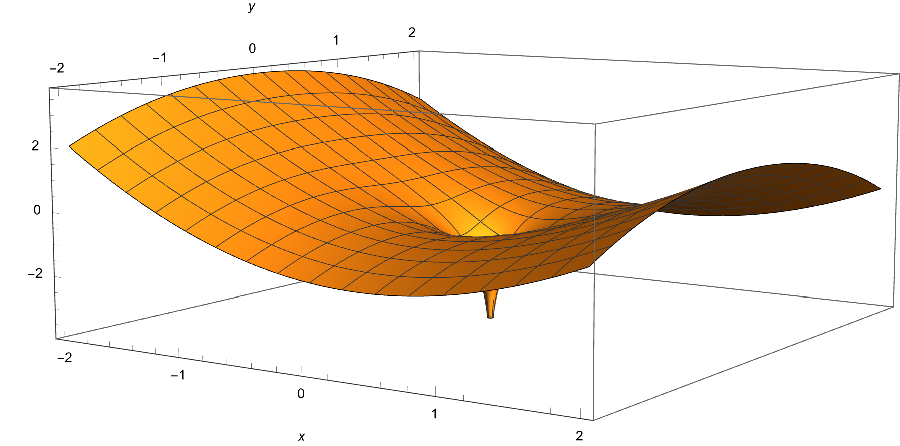
\includegraphics[height=.3\textwidth]{pictures/ReS_imaginary_3D.pdf}
	\qquad
	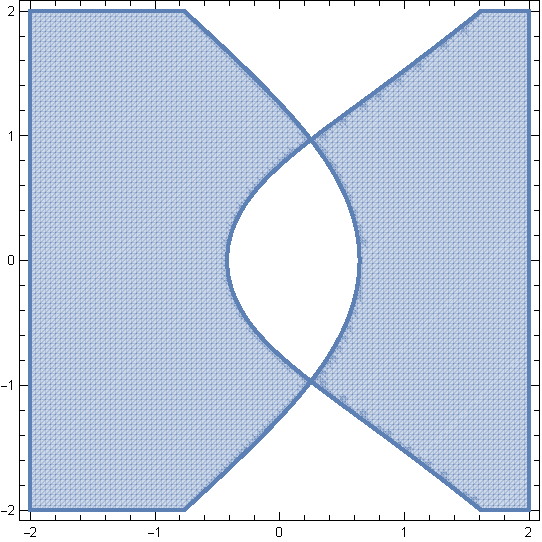
\includegraphics[height=.3\textwidth]{pictures/ReS_imaginary_region.pdf}
	\caption{A 3D plot and a region plot of the
	regions where $\operatorname{Re}S(z)-\operatorname{Re}S(z_{cr})$ is positive
	(highlighted) or negative, in the case $X=\frac{1}{2}$.
	In this case, $z_{cr}\approx 0.25+0.96 i$.}
	\label{fig:ReS_imaginary}
\end{figure}

From the region plot, we see that the new $z$ contour should
pass through the shaded region $\operatorname{Re}S(z)-\operatorname{Re}S(z_{cr})>0$,
and the new $w$ contour should pass through the unshaded region
$\operatorname{Re}S(z)-\operatorname{Re}S(z_{cr})<0$.

Deforming the contours from \Cref{fig:contours} to the new contours
is impossible without passing through the residue at $w=z$.
Moreover, this residue appears only for certain values of $z$. Namely, for $X=0$,
let us first make the $z$ contour to be the positively (counterclockwise) oriented
unit circle.
It passes through the critical points $z_{cr}=i$ and $\overline{z_{cr}}=-i$.
Since the original $w$ contour is to the right of the $z$ contour, we only
encounter the residue when $z$ is in the right half of the circle.

Thus, we can write
\begin{equation}
	\label{eq:K_n_bulk_deformation}
	\oiint_{\textnormal{old contours}}=
	\oiint_{\textnormal{new contours}}
	+
	\int_{-i}^i 2\pi i\ssp \operatorname{Res}\limits_{w=z}\ssp dz,
\end{equation}
where in the single integral, the $z$ contour passes to the right of the origin,
along the right half of the unit circle.

It remains to consider the two integrals in the right-hand side
of \eqref{eq:K_n_bulk_deformation}.
Recall that the correlation functions are
defined relative to a reference measure, and the right object to scale is
\begin{equation*}
	K_n(x,y)dy=\frac{1}{\sqrt n}\ssp d\left( \Delta y \right).
\end{equation*}
The extra factor $n^{-1/2}$
compensates the prefactor $\sqrt n$ in
\eqref{eq:K_n_scaling}.

The single integral takes the form
\begin{equation}
	\label{eq:K_n_bulk_single}
	\frac{-i}{2\pi}
	\int_{-i}^i
	e^{z (\Delta x -\Delta y)}
	\ssp
	dz
	=\frac{\sin\left( \Delta x-\Delta y \right)}{\pi(\Delta x-\Delta y)},
	\qquad \Delta x,\Delta y\in\mathbb{R}.
\end{equation}
\begin{definition}
	\label{def:sine-kernel}
	The \emph{sine kernel} is defined as
	\begin{equation*}
		K_{\mathrm{sine}}(x,y)\coloneqq
		\begin{cases}
			\dfrac{\sin (x-y)}{\pi (x-y)},&\qquad x\ne 0,\\[10pt]
			\dfrac{1}{\pi},&\qquad x=0.
		\end{cases}
	\end{equation*}
	(The value at $x=y$ is defined by continuity.)

	This kernel is translation invariant, and is often
	defined with a single argument, as
	$K_{\mathrm{sine}}(x-y)$.
\end{definition}

The double integral has both contours
in the ``steepest descent'' regime, which means that
the main contribution is
\begin{equation*}
	\mathrm{const}\cdot
	\frac{e^{n\left( \operatorname{Re}S(z_{cr})-\operatorname{Re}S(z_{cr}) \right)}}{\sqrt n}
	\sim \frac{\mathrm{const}}{\sqrt n}.
\end{equation*}
At this rate, the double integral over the new contours
\emph{does not} contribute to the asymptotics of the correlation functions.
Recall that the correlation functions are expressed as finite-dimensional
determinants of the kernel $K_n(x,y)$, and the error $O(n^{-1/2})$ is
negligible in the limit $n\to+\infty$.
This is because the main term comes from the single integral,
which does not vanish.

We have established the following result:
\begin{proposition}[Bulk asymptotics at $X=0$]
	\label{prop:bulk}
	The correlation kernel $K_n$ of the GUE has the following asymptotics
	close to zero as $n\to+\infty$:
	\begin{equation*}
		\lim_{n\to \infty}
		\frac{1}{\sqrt n}
		K_n\left( \frac{\Delta x}{\sqrt n},\frac{\Delta y}{\sqrt n} \right)
		=
		K_{\mathrm{sine}}\left( \Delta x,\Delta y \right),
		\qquad \Delta x,\Delta y\in\mathbb{R}.
	\end{equation*}
	Consequently, the eigenvalues of the GUE converge to the sine process
	determined by the sine kernel (\Cref{def:sine-kernel}),
	in the sense of finite-dimensional distributions.
\end{proposition}

\begin{remark}
	Beyond $X=0$, the local correlations are essentially the same,
	up to rescaling of the real line by a constant factor (depending
	on the semicircle density).
	See Problem~\ref{prob:imaginary-critical-points}.
\end{remark}

\subsection{Real critical points: $|X|>2$, ``large deviations''}
\label{sub:real-critical-points}

For \(X^2>4\), both solutions
\eqref{eq:critical-points}
are real. Let us assume $X>2$, the case \(X<2\) is similar.
For $X>2$, both solutions are positive.
Label these solutions as
\[
	z_+ \;=\;\frac{X + \sqrt{X^2-4}}{2},
	\qquad
	z_- \;=\;\frac{X - \sqrt{X^2-4}}{2},
	\quad
	\text{so that}\quad z_+z_-=1.
\]
A straightforward check reveals that \(z_+\!>\!1\) and \(z_-\!<\!1\) (for \(X>2\)).
Note that $S''(z)=1-z^{-2}$, which is positive for \(z_+>1\) and negative for \(z_-<1\).  Thus, the critical points \(z_+\) and \(z_-\) are a local minimum and a local maximum.
A crucial observation is that
\begin{equation*}
	S(z_+)<S(z_-).
\end{equation*}
One can deform the $z$ integration contour to pass through
$z_-$ and the $w$ contour to pass through $z_+$.
Then, on these contours, one can show that
\begin{equation*}
	\operatorname{Re}S(w)-\operatorname{Re}S(z)<0.
\end{equation*}
According to the steepest descent ideology,
we see that the main exponential behavior of the double contour integral is
\begin{equation}
	\label{eq:Oexp}
	\exp\left\{ n\left(
		\operatorname{Re}S(z_+)-\operatorname{Re}S(z_-)
\right) \right\}=O( e^{-\delta(X)n} ), \qquad |X|>2.
\end{equation}
Here $\delta(X)>0$ for $|X|>2$, and $\delta(X)\to0$ when $|X|\to2$.

The outcome \eqref{eq:Oexp} reflects the fact that the
Wigner semicircle law places all eigenvalues inside the
interval \(\lvert X\rvert \le 2\).
The probability to see even a single eigenvalue outside $[-2,2]$
is exponentially small.

This exponential decay corresponds to a large deviation regime.
Indeed, if at least one of the diagonal entries of the matrix
is unusually large, this corresponds to
the maximal eigenvalue to get outside the interval \([-2,2]\).
See also Problem~\ref{prob:large-deviation}.


\subsection{Double critical point: $|X|=2$, ``edge''}
\label{sub:double-critical-points}

Throughout the subsection, we assume that $X=2$. The case $X=-2$ is symmetric.

When \(X=2\), the two solutions in \eqref{eq:critical-points} merge into a double critical point
$z_{cr}=1$.
We have
\[
S'(1)=0,\qquad S''(1)=0,\qquad S'''(1)=2.
\]
Thus, the usual quadratic approximation fails and one must expand to third order. Writing
\[
z=1+u,\qquad w=1+v,
\]
with \(u,v\) small, we have
\[
S(1+u)=S(1)+\frac{S'''(1)}{6}\,u^3+O(u^4)
=S(1)+\frac{u^3}{3}+O(u^4),
\]
and similarly for \(S(1+v)\). Hence, the difference in the exponents becomes
\[
S(1+v)-S(1+u)=\frac{v^3-u^3}{3}+O(u^4+v^4).
\]

To capture the correct asymptotics, we rescale the local variables by setting
\[
u=\frac{U}{n^{1/3}},\qquad v=\frac{V}{n^{1/3}},
\]
so that
\[
n\Bigl[S(1+v)-S(1+u)\Bigr]=\frac{V^3-U^3}{3}+O\Bigl(n^{-1/3}\Bigr).
\]
Moreover, the correct edge scaling for the spatial variables is obtained by writing
\[
x=2\sqrt{n}+\frac{\xi}{n^{1/6}},\qquad y=2\sqrt{n}+\frac{\eta}{n^{1/6}},\qquad \xi,\eta\in\mathbb{R}.
\]
We have
\begin{equation*}
	n\left( S(w)-S(z) \right)=n^{1/3}(\xi-\eta)+
	\frac{V^3-U^3}{3}+\xi U-\eta V+O\Bigl(n^{-1/3}\Bigr).
\end{equation*}
The terms $n^{1/3}(\xi-\eta)$ are harmless as they can be removed
by conjugation.

The region plot of $\operatorname{Re}S(z)-\operatorname{Re}S(1)$
(shown in \Cref{fig:ReS_edge})
makes sure that we can deform the $z$ contour so that it passes through $z_{cr}=1$
as the new $U$ contour at the angles $\pm \frac{2\pi}{3}$ (where $\operatorname{Re}U^3>0$),
we can deform the $w$ contour so that it passes through $z_{cr}=1$
as the new $V$ contour at the angles $\pm \frac{\pi}{3}$ (where $\operatorname{Re}V^3<0$).
This will ensure the convergence of the new double integral.

\begin{figure}[htpb]
	\centering
	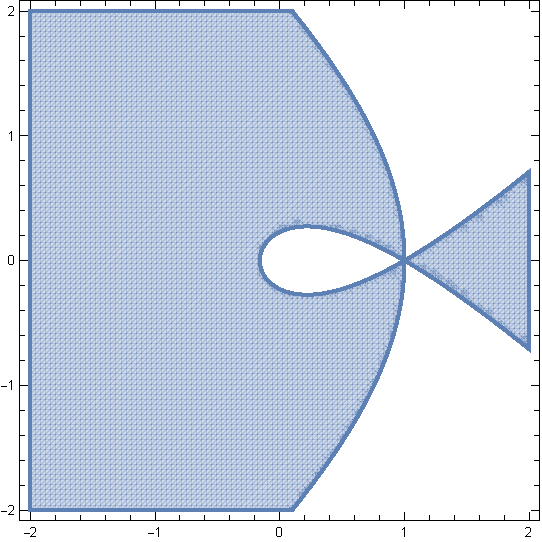
\includegraphics[height=.3\textwidth]{pictures/ReS_edge.pdf}
	\caption{The plot of the region $\operatorname{Re}S(z)-\operatorname{Re}S(1)>0$ for $X=2$.}
	\label{fig:ReS_edge}
\end{figure}

Thus, we have shown that under the rescaling, the GUE correlation kernel
$K_n(x,y)\ssp dy$ converges to a new kernel.
\begin{definition}
	\label{def:Airy_kernel}
	Define the \emph{Airy kernel} on $\mathbb{R}$ by
	\begin{equation*}
		K_{\mathrm{Ai}}(\xi,\eta)=\frac{1}{(2\pi i)^2}
		\int_{e^{-\frac{\pi i}{3}}\infty}^{e^{\frac{\pi i}{3}}\infty}dV
		\int_{e^{-\frac{2\pi i}{3}}\infty}^{e^{2\frac{\pi i}{3}}\infty}dU
		\ssp
		\frac{\exp\Bigl\{\frac{V^3-U^3}{3}+U\,\xi-V\,\eta\Bigr\}}{V-U}.
	\end{equation*}
	For another formula for the Airy kernel
	which does not involve integrals,
	see
	Problem~\ref{prob:airy}.
\end{definition}

\begin{proposition}
	\label{prop:edge}
	We have
	\begin{equation*}
		\lim_{n\to\infty}
		\frac{1}{n^{1/6}}K_n\Bigl(2\sqrt{n}+\frac{\xi}{n^{1/6}},\,2\sqrt{n}+\frac{\eta}{n^{1/6}}\Bigr)
		\to
		K_{\mathrm{Ai}}(\xi,\eta).
	\end{equation*}
	Consequently, the eigenvalue statistics at the edge of the spectrum converge to the Airy point process, in the sense of fine-dimensional distributions.
\end{proposition}

\subsection{Airy kernel, Tracy--Widom distribution, and convergence of the maximal
eigenvalue}

Let us make a few remarks on the asymptotic results of
\Cref{prop:bulk,prop:edge}.
First,
a rigorous justification of convergence
of contour integrals requires some estimates on the error terms
in the steepest descent analysis, but these
estimates are mild and not hard to obtain.

Second, the GUE has the maximal eigenvalue $\lambda_{max}$. It is reasonable
to assume that the Airy process also (almost surely) admits a maximal point
(usually denoted by $\mathfrak{a}_1$),
and that $\lambda_{max}$
converges to $\mathfrak{a}_1$ under appropriate rescaling:
\begin{equation}
	\label{eq:TW_GUE}
	\lim_{n\to\infty}n^{\frac{1}{6}}\bigl(\lambda_{max}-2\sqrt{n}\bigr)=\mathfrak{a}_1.
\end{equation}
This is indeed the case, but to show \eqref{eq:TW_GUE}, one needs to
show the convergence in distribution:
\begin{equation}
	\label{eq:TW_GUE_convergence}
	\lim_{n\to \infty}
	\mathbb{P}\Bigl(n^{1/6}(\lambda_{max}-2\sqrt{n})\le x\Bigr)
	\to
	\mathbb{P}(\mathfrak{a}_1\le x).
\end{equation}
Both events \eqref{eq:TW_GUE_convergence} are so-called
\emph{gap probabilities}, for example,
\begin{equation*}
	\operatorname{P}(\mathfrak{a}_1\le x)=
	\operatorname{P}(\textnormal{there are no eigenvalues in the interval $(x,\infty)$}),
\end{equation*}
which is expressed as
the Fredholm determinant
\begin{equation}
	\label{eq:gap-probability-Ai-Fredholm}
	\det\left( 1-K_{\mathrm{Ai}} \right)_{(x,\infty)}=
	1+\sum_{m=1}^{\infty}\frac{(-1)^m}{m!}
	\int_x^{\infty}dy_1\int_x^{\infty}dy_2\cdots
	\int_x^{\infty}dy_m
	\ssp
	\det\limits_{i,j=1}^m
	K_{\mathrm{Ai}}(y_i,y_j).
\end{equation}
Thus, to get \eqref{eq:TW_GUE_convergence}), one needs to show the convergence
of sums like this for the GUE kernel
to the corresponding sums for the Airy kernel. This is doable, but tedious.

Moreover, to get convergence in distribution of random variables,
one would also have to argue either \emph{tightness},
or independently show that
\eqref{eq:gap-probability-Ai-Fredholm} defines a
cumulative probability
distribution function in $x$:
\begin{equation}
	\label{eq:TW_GUE_cdf}
	F_2(x)=\det\left( 1-K_{\mathrm{Ai}} \right)_{(x,\infty)}.
\end{equation}
The distribution \eqref{eq:TW_GUE_cdf} is known as the \emph{GUE Tracy--Widom distribution}.
The subscript $2$ indicates that $\beta=2$. There are distributions
$F_\beta$ for all beta, most notably, the GOE and GSE distributions.
The classical distributions $F_1,F_2,F_4$ also appear as fluctuation distributions
in interacting particle systems, while other beta values do
not quite appear in the particle systems
domain.

More details
may be found in the original papers
\cite{tracy1993level},
\cite{Forrester1993},
\cite{tracy_widom1994level_airy}.





%%%%%%%%%%%%%%%%%%%%%%%%%%%%%%%%%%%%%%%%%%%%%%%%%%%%%%%%%%%%
\section{Introduction and Motivation}


In random matrix theory, one often studies the entire spectrum of an $n\times n$ matrix ensemble such as the Gaussian Unitary Ensemble (GUE), the Gaussian Orthogonal Ensemble (GOE), or, more generally, $\beta$-ensembles. However, it is also natural to examine the spectra of \emph{principal minors} of such matrices.

When we say ``cutting corners,'' we typically refer to extracting a top-left $k\times k$ submatrix (or \emph{corner}) out of an $n\times n$ random matrix $H$ and then looking at the interplay among the eigenvalues of all corners $k=1,\dots,n$. This forms a \emph{nested} family of spectra, often described by interlacing (or Gelfand--Tsetlin) patterns.

The \emph{GUE corners process} is a classical example of this phenomenon. Concretely, if $H$ is an $n\times n$ GUE matrix, then the top-left $k\times k$ corners (for $1\le k\le n$) have jointly distributed eigenvalues that exhibit remarkable determinantal structures, interlacing inequalities, and limit theorems. Similar statements hold for the GOE, the Gaussian Symplectic Ensemble (GSE), and more general $\beta$-ensembles (algebraic generalizations of GUE/GOE/GSE that we also discuss).

\subsection{Outline}
These notes proceed as follows:
\begin{itemize}
\item[\S\ref{sec:preliminaries}] \textbf{Preliminaries.} We recall the GUE definition, its diagonalization, and the general $\beta$-ensembles.
\item[\S\ref{sec:corners-definition}] \textbf{Corners of Random Matrices.} We define the corner (minor) processes and recall the fundamental interlacing property.
\item[\S\ref{sec:gue-corners}] \textbf{GUE Corners: Joint Distribution and Determinantal Structure.} We outline how to compute the joint distribution of the spectra of all corners, show the interlacing, and discuss the determinantal kernel.
\item[\S\ref{sec:generalbeta}] \textbf{General $\beta$ Corners.} We show how the GUE corners result has a natural extension to the tridiagonal $\beta$-ensembles (Dumitriu--Edelman) and mention connections to Wishart/Laguerre and Jacobi corners.
\item[\S\ref{sec:local-limits}] \textbf{Local Limits.} We review the bulk (sine) and edge (Airy) universality in each corner and highlight how the entire triangular array has consistent local limits.
\item[\S\ref{sec:applications}] \textbf{Connections and Applications.} We discuss ties to Gelfand--Tsetlin patterns, representation theory, partial Haar unitaries, and beyond.
\item[\S\ref{sec:problems}] \textbf{Exercises.} We present problem sets illustrating these concepts.
\end{itemize}

%%%%%%%%%%%%%%%%%%%%%%%%%%%%%%%%%%%%%%%%%%%%%%%%%%%%%%%%%%%%
\section{Preliminaries on Gaussian and $\beta$-Ensembles}
\label{sec:preliminaries}

\subsection{GUE Definition and Basic Facts}
The Gaussian Unitary Ensemble (GUE$_n$) is the probability distribution on $n\times n$ Hermitian matrices whose density is proportional to
\[
	\exp\Bigl(-\tfrac{1}{2}\,\mathrm{Tr}(H^2)\Bigr)\,dH,
\]
where $dH$ denotes the Lebesgue measure on the space of Hermitian $n\times n$ matrices. Equivalently, one can specify that the entries $H_{ij}$ for $i<j$ are i.i.d.\ complex Gaussians with mean zero and variance $1/2$, and the diagonal entries $H_{ii}$ are i.i.d.\ real Gaussians with mean zero and variance $1$.

A fundamental property is that the joint distribution of eigenvalues $(\lambda_1,\dots,\lambda_n)$ (ordered in any way, typically $\lambda_1\ge \cdots \ge \lambda_n$) is given by the well-known \emph{Hermite (or GUE) $\beta=2$-ensemble} formula:
\begin{equation}\label{eq:gue-eig-pdf}
	p(\lambda_1,\dots,\lambda_n)
	\;=\;\frac{1}{Z_{n}}
	\prod_{i<j}(\lambda_i-\lambda_j)^2
	\exp\Bigl(-\tfrac{1}{2}\sum_{k=1}^n\lambda_k^2\Bigr).
\end{equation}
Here $Z_n$ is the normalizing constant. The $\beta=2$ in the exponent of the Vandermonde product $\prod_{i<j}(\lambda_i-\lambda_j)^\beta$ reflects the unitary symmetry class.

\subsection{General $\beta$-Ensembles}
\label{sec:beta-ensembles}
More generally, one can define a one-parameter family of ensembles indexed by $\beta>0$, called \emph{$\beta$-ensembles}:
\begin{equation}\label{eq:beta-pdf}
	p_\beta(\lambda_1,\dots,\lambda_n)
	\;=\;\frac{1}{Z_{n,\beta}}
	\prod_{i<j}\!|\lambda_i-\lambda_j|^\beta
	\prod_{k=1}^n e^{-V(\lambda_k)},
\end{equation}
where $V(x)$ is a confining potential, often taken as $V(x)=\tfrac{x^2}{2}$ (Gaussian case) or $V(x)$ suitable for other classical ensembles (e.g., Laguerre/Wishart, Jacobi, etc.). For $\beta=1,2,4$ these correspond to the classical GOE, GUE, GSE, respectively, but $\beta$ need not be an integer or even rational.

An important way to realize the $\beta$-ensembles (with Gaussian potential) is via the \emph{Dumitriu--Edelman} tridiagonal representation: one constructs an $n\times n$ tridiagonal matrix $T_\beta$ whose diagonal entries are i.i.d.\ Gaussians (with certain means and variances) and whose sub- and super-diagonal entries are independent $\chi$-distributed random variables. For $\beta=2$, this recovers the GUE tridiagonal matrix. All of these $\beta$-ensembles share the fundamental property that their eigenvalues form a \emph{repulsive point process} governed by \eqref{eq:beta-pdf}.

%%%%%%%%%%%%%%%%%%%%%%%%%%%%%%%%%%%%%%%%%%%%%%%%%%%%%%%%%%%%
\section{Corners of Hermitian Matrices: Definition and Interlacing}
\label{sec:corners-definition}

\subsection{Principal Corners (Minors)}
Let $H$ be an $n\times n$ Hermitian matrix. For each $1\le k\le n$, define the \emph{top-left $k\times k$ corner} $H^{(k)}$ by
\[
	H^{(k)} \;=\; \bigl[H_{ij}\bigr]_{1\le i,j \le k}.
\]
Since $H$ is Hermitian, each $H^{(k)}$ is also Hermitian. Let
\[
	\lambda_1^{(k)} \;\ge\;\lambda_2^{(k)}\;\ge\;\cdots\;\ge\;\lambda_k^{(k)}
\]
denote the eigenvalues of $H^{(k)}$. Then the collection
\[
	\bigl\{\lambda_j^{(k)} : 1\le j\le k \le n\bigr\}
\]
is called the \emph{corners spectrum} (or \emph{minor spectrum}) of $H$. When $H$ is random, this entire triangular array of eigenvalues becomes a random point configuration in the two-dimensional set $\{1,\dots,n\}\times \mathbb{R}$.

\subsection{Interlacing Property}
A fundamental feature of Hermitian matrices is that the eigenvalues of corners interlace with the eigenvalues of the full matrix. More precisely, if $\nu_1\ge\dots\ge \nu_n$ are the eigenvalues of $H$ itself (i.e., the full $n\times n$ matrix), and $\mu_1\ge\cdots\ge\mu_k$ are the eigenvalues of $H^{(k)}$, then we have:
\[
	\nu_1\;\ge\;\mu_1\;\ge\;\nu_2\;\ge\;\mu_2\;\ge\;\dots\;\ge\;\nu_k\;\ge\;\mu_k\;\ge\;\nu_{k+1}.
\]
In particular,
\[
	\lambda_1^{(k+1)}
	\;\le\;\lambda_1^{(k)}\;\le\;\lambda_2^{(k+1)}
	\;\le\;\cdots\;\le\;\lambda_k^{(k)}
	\;\le\;\lambda_{k+1}^{(k+1)}.
\]
Graphically, one can depict $\{\lambda_j^{(k)}\}$ in a triangular Gelfand--Tsetlin pattern form, reflecting these interlacing inequalities.

\begin{remark}[Schur Complement Interpretation]
The interlacing property can be seen via Schur complements: when passing from $H$ to its $(n-1)\times(n-1)$ corner, one effectively removes the last row and column, so the rank-one update in the Schur complement triggers the Weilandt--Hoffman/Cauchy interlacing inequalities.
\end{remark}

%%%%%%%%%%%%%%%%%%%%%%%%%%%%%%%%%%%%%%%%%%%%%%%%%%%%%%%%%%%%
\section{GUE Corners: Joint Distribution and Determinantal Structure}
\label{sec:gue-corners}

Consider now the \emph{joint} distribution of all corners of a GUE$_n$ matrix $H$. That is, we have the random matrices
\[
	H^{(1)},\,H^{(2)},\,\dots,\,H^{(n)}=H,
\]
and want to understand the collection $\{\lambda_j^{(k)}\}$ for $1\le j\le k\le n$ as a single random point process.

\subsection{Spectral Decomposition and Haar Unitary}
Recall that $H$ can be diagonalized:
\[
	H = U \Lambda U^\dagger,
	\quad
	\Lambda = diag(\lambda_1,\dots,\lambda_n),
\]
where $\Lambda$ is the real diagonal matrix of $H$'s eigenvalues (in descending order) and $U$ is Haar-distributed on the unitary group $\mathrm{U}(n)$. The top-left $k\times k$ corner $H^{(k)}$ can be written in terms of sub-blocks of $U$ and $\Lambda$. In principle, one then integrates over the Haar measure to derive the joint law of $(H^{(1)},\dots,H^{(n)})$.

While the resulting distribution is complicated, it is nevertheless highly structured and, in fact, forms a \emph{determinantal point process} (DPP) in the two-dimensional space of ``row index $k$'' and ``spectral variable $x$.''

\subsection{Determinantal Form: GUE Corners Process}
The formal statement (see, e.g., \cite{Johansson-2005,Johansson-2006,baryshnikov2001gues,forrester2010log} for references) is:

\begin{theorem}[GUE Corners as a 2D Determinantal Process]
\label{thm:gue-corners-det}
Let $H$ be an $n\times n$ GUE matrix and let $\{\lambda_j^{(k)}\}_{1\le j\le k\le n}$ be the eigenvalues of its top-left corners of sizes $k=1,\dots,n$. Then, viewed as a random point set in $\{1,\dots,n\}\times\mathbb{R}$, this collection is a \emph{determinantal point process}:
\[
	\mathbb{P}\bigl[(k_1,x_1),\dots,(k_m,x_m)\in \text{the process}\bigr]
	= \det\!\Bigl[K\bigl((k_i,x_i),(k_j,x_j)\bigr)\Bigr]_{i,j=1}^m,
\]
where $K$ is the \emph{extended correlation kernel}. In particular, correlation functions for the entire triangular array are given by minors of $K$.
\end{theorem}

Explicit formulas for $K\bigl((k,x),(k',y)\bigr)$ exist, but are somewhat more involved than the single-size GUE kernel. Nevertheless, one can still identify them in terms of \emph{orthogonal polynomials} (Hermite polynomials) and certain additional matrix integrals.

\begin{remark}
For $k=n$ (the largest corner), we recover the usual 1D GUE correlation kernel restricted to the $\lambda_i^{(n)}$ alone. The extended 2D kernel encapsulates how these GUE eigenvalues relate to the smaller corners.
\end{remark}

\subsection{Gelfand--Tsetlin Patterns and Markov Structure}
An important combinatorial viewpoint: if we only keep track of the eigenvalues (without any concern for eigenvectors), the random array $\{\lambda_j^{(k)}\}$ forms a random Gelfand--Tsetlin pattern with continuous entries. One can show that as $k$ increases, $(\lambda_1^{(k)},\dots,\lambda_k^{(k)})$ is a \emph{Markov chain} in $k$:
\[
	(\lambda_1^{(1)})
	\;\longrightarrow\;
	(\lambda_1^{(2)},\lambda_2^{(2)})
	\;\longrightarrow\;
	\cdots
	\;\longrightarrow\;
	(\lambda_1^{(n)},\dots,\lambda_n^{(n)}).
\]
The transition density from $(k)$-corner eigenvalues to $(k+1)$-corner eigenvalues encodes the interlacing constraints and the GUE invariance. Determinantal structure yields closed-form transition kernels.

%%%%%%%%%%%%%%%%%%%%%%%%%%%%%%%%%%%%%%%%%%%%%%%%%%%%%%%%%%%%
\section{General $\beta$ Corners Processes}
\label{sec:generalbeta}

The GUE case ($\beta=2$) is the richest in integrable (determinantal) structures, but corners processes exist for all $\beta$ as well. Specifically, if one considers the $\beta$-ensemble in tridiagonal form (the Dumitriu--Edelman approach), then the top-left corners of this tridiagonal matrix yield an entire nested sequence of $\beta$-ensembles for smaller dimensions, though with certain correlated modifications. The full joint distribution of all these corners forms a random triangular array with similar \emph{interlacing} constraints. The structure is no longer purely determinantal for general $\beta$, but it can often be described via \emph{multivariate Bessel functions}, \emph{Selberg integrals}, or other integrable-type objects depending on $\beta$.

For example:
\begin{itemize}
\item In the \emph{Gaussian Orthogonal Ensemble} ($\beta=1$), the corners process has a Pfaffian structure (due to real symmetry and real eigenvectors).
\item In the \emph{Gaussian Symplectic Ensemble} ($\beta=4$), a related Pfaffian structure appears (with symplectic symmetry).
\item For general $\beta$, corners processes can often be described by hypergeometric functions of matrix arguments, or can be seen as special cases of the so-called \emph{multivariate hypergeometric orthogonal polynomial ensembles}.
\end{itemize}
Thus, while $\beta=2$ remains the simplest and most explicit (due to unitarity and determinantal formulas), the phenomenon of ``cutting corners'' to get a nested set of minors is pervasive across all $\beta$.

\subsection{Wishart/Laguerre and Jacobi Corners}
Similar statements hold for Wishart (Laguerre) ensembles or Jacobi (MANOVA) ensembles. One can look at partial corners, say the top-left corner of a rectangular Gaussian matrix $X$, or the principal corners of $X^\dagger X$ (Wishart), or the corners of a random unitary sub-block (Jacobi). The spectra and their interlacing relationships again produce a random triangular array with a structured correlation law. These corner processes are widely studied in multivariate statistics and in representation-theoretic random measures.

%%%%%%%%%%%%%%%%%%%%%%%%%%%%%%%%%%%%%%%%%%%%%%%%%%%%%%%%%%%%
\section{Local Limits: Bulk and Edge of Each Corner}
\label{sec:local-limits}

One might ask how the local eigenvalue statistics for smaller corners compare to those in the full matrix. Indeed, each corner $H^{(k)}$ is a $k\times k$ Hermitian matrix, so in the limit $n\to\infty$ (and possibly $k\to\infty$ in tandem with $n$), we can look at:
\[
	\lambda_{\max}^{(k)},\quad
	\text{gap statistics in the interior of the spectrum of }H^{(k)},\dots
\]
An interesting scenario is when $k$ is proportional to $n$, i.e.\ $k=\alpha n$ for some $0<\alpha\le1$. For the GUE, one can use known results about \emph{rank-one updates} or the fact that $H^{(k)}$ is close (in a certain sense) to a smaller GUE plus correlated terms. The main takeaway is that:
\begin{itemize}
	\item The \emph{global} empirical distribution of $H^{(k)}$ converges to the Wigner semicircle (or appropriate portion of it) if $k\to\infty$. In fact, as $k,n\to\infty$ with $k/n\to\alpha$, the top-left corners have a limiting spectral distribution that is the same as the GUE scaled by $\sqrt{n}$, up to small boundary effects.
\item The \emph{local} statistics in the bulk remain universal, giving the \emph{sine kernel} limit. Near the edge, we get \emph{Airy} behavior. These corners do not break the usual universality phenomena: local fluctuations around scaled spectral points still follow the same universal kernels.
\item There are also interesting \emph{transitional} regimes if $k$ is close to $n$, or if $k$ is fixed while $n\to\infty$. In the latter case, $H^{(k)}$ does not grow in size, so the distribution of the $k\times k$ corner can converge to that of a simpler random matrix ensemble with additional constraints.
\end{itemize}
Hence, one sees a consistent story: the entire triangular array $\{\lambda_j^{(k)}\}$ has local limits that are consistent with the well-known universal kernels in random matrix theory.

%%%%%%%%%%%%%%%%%%%%%%%%%%%%%%%%%%%%%%%%%%%%%%%%%%%%%%%%%%%%
\section{Connections and Applications}
\label{sec:applications}

\subsection{Gelfand--Tsetlin Patterns in Representation Theory}
The corner spectra of a GUE matrix can be viewed as generating a random Gelfand--Tsetlin pattern in continuous variables:
\[
	\begin{matrix}
	\lambda_1^{(n)} \\
	\lambda_1^{(n-1)} & \lambda_2^{(n-1)} & \dots & \lambda_{n-1}^{(n-1)} \\
	\vdots & & \ddots & \vdots \\
	\lambda_1^{(1)}
	\end{matrix}
\]
with $\lambda_{j}^{(k)}\ge \lambda_{j+1}^{(k+1)}\ge \cdots$. This is directly analogous to the discrete Gelfand--Tsetlin patterns that parametrize irreducible representations of $\mathrm{U}(n)$ (or $\mathrm{SU}(n)$). The random matrix approach suggests that these continuous patterns are natural objects carrying determinantal/Pfaffian structures, leading to connections with \emph{asymptotic representation theory} and \emph{integrable probability}.

\subsection{Partial Haar Unitaries}
If $H=U\Lambda U^\dagger$ with $U$ Haar-distributed on $\mathrm{U}(n)$, then the sub-blocks of $U$ (e.g., the top-left $k\times n$ portion) inherit special rotational invariance properties known as \emph{partial Haar unitaries} or \emph{isometries} from the group measure. One can interpret the corners $H^{(k)}$ in terms of these partial unitaries. This viewpoint is used in quantum information (for random states and channels) and in multivariate statistics (for random orthonormal bases).

\subsection{Integrable Systems and Discrete Analogs}
Finally, corners processes appear in integrable models of lattice systems and random partitions. For instance, certain \emph{plane partitions} or \emph{Young tableaux} ensembles have limiting shapes described by the GUE-corners distribution in scaled coordinates. The broad principle is that any strongly \emph{interlacing} or \emph{Gelfand--Tsetlin} structure with underlying determinantal or Pfaffian formula often is governed by the same universal corners processes seen in random matrix theory.

%%%%%%%%%%%%%%%%%%%%%%%%%%%%%%%%%%%%%%%%%%%%%%%%%%%%%%%%%%%%
\section{Problems and Exercises}
\label{sec:problems}

\begin{enumerate}
\item \textbf{Schur Complement and Interlacing.} \\
Given a Hermitian matrix $A$ of size $n\times n$, show that its $(n-1)\times(n-1)$ top-left corner $A^{(n-1)}$ is the Schur complement obtained by removing the last row/column. Use this viewpoint to deduce the interlacing property between the eigenvalues of $A^{(n-1)}$ and $A$.
\medskip

\item \textbf{Determinantal / Pfaffian Structures for $\beta=1,2,4$.} \\
Explain why for $\beta=1,4$ (the GOE and GSE), one gets \emph{Pfaffian} structures rather than purely determinantal ones. Sketch how the presence of real symmetry ($\beta=1$) or symplectic symmetry ($\beta=4$) modifies the joint law of eigenvalues.
\medskip

\item \textbf{GUE Corners for $n=2$ and $n=3$.} \\
Explicitly write out (symbolically, or with a small calculation) the joint distribution of $\{\lambda^{(k)}_j\}$ for $k=1,2$ (when $n=2$), and similarly for $n=3$. Identify how the interlacing $\lambda_1^{(1)}\ge \lambda_1^{(2)}\ge \lambda_2^{(2)}$ appears. Check if you can see any determinant form for correlation functions in these small cases.
\medskip

\item \textbf{Tridiagonal Realization of Corners ($\beta=2$).} \\
Construct a tridiagonal GUE matrix $T$ of size $n$, then look at the principal $(k\times k)$ top-left submatrix $T^{(k)}$. Compare the distribution of $T^{(k)}$ with that of a smaller GUE(\!$k$) matrix. Are they the same or different? If different, precisely how do they differ?
\medskip

\item \textbf{Wishart / Laguerre Corners.} \\
Consider the Wishart/Laguerre ensemble $W = X^\dagger X$, where $X$ is an $m\times n$ complex Gaussian matrix. Define $W^{(k)}$ as the top-left $k\times k$ corner. Write out the joint distribution of eigenvalues of $W^{(1)},\dots,W^{(n)}$ (assuming $m\ge n$). Describe the interlacing properties and how they relate to the GUE corners for a suitable transformation of $W$.
\medskip

\item \textbf{Local Limit for a Fixed-Size Corner.} \\
For a large $n\times n$ GUE, consider only the top-left $k\times k$ corner for some \emph{fixed} $k$. Show that in the $n\to\infty$ limit, this corner \emph{converges in distribution} to a simpler random matrix (explain or guess its form). Does this limit matrix have i.i.d.\ entries? Discuss the effect of the rank-1 update from the rest of the matrix.
\medskip

\item \textbf{Markov Property in the Triangular Array.} \\
Prove (or outline why) the sequence of eigenvalue vectors $(\lambda_1^{(k)},\dots,\lambda_k^{(k)})$ is a Markov chain in $k$, for the GUE corners process. Determine the transition kernel in the finite $n$ case or give a reference for its explicit form.
\end{enumerate}





































\appendix
\setcounter{section}{6}

\section{Problems (due 2025-03-25)}

\subsection{Airy kernel}
\label{prob:airy}

Define the Airy function by
\begin{equation*}
	Ai(\xi)\coloneqq
	\frac{1}{2\pi}\int_{-\infty}^\infty
	e^{i U^3/3+i\xi U} dU=
	\frac{1}{\pi}\int_0^\infty
	\cos\left( \frac{U^3}{3}+\xi U \right)\ssp dU.
\end{equation*}
This integral converges, but only conditionally. To improve convergence,
one should instead integrate
along a complex contour,
from $e^{\frac{5 \pi i}{6}}\infty$ to $0$ to
$e^{\frac{\pi i}{6}}\infty$.

Show that
\begin{equation*}
	K_{\mathrm{Ai}}(\xi,\eta)=
	\frac{Ai(\xi)\ssp Ai'(\eta)-Ai(\eta)\ssp Ai'(\xi)}{\xi-\eta}.
\end{equation*}
Note that this expression is parallel to the sine kernel,
\begin{equation*}
	\frac{\sin(x-y)}{\pi(x-y)}=\frac{\sin x\cos y-\cos x\sin y}{\pi(x-y)},\qquad
	\cos x=(\sin x)'.
\end{equation*}
These correlation kernels are called \emph{integrable}
\cite{its1990differential}.

Hint for the problem: observe that
\begin{equation*}
	\exp\left\{ -i z x+iwy \right\}=\frac{i}{x-y}\left( \frac{\partial}{\partial z}+
	\frac{\partial}{\partial w}\right)\exp\left\{ -i z x+iwy \right\},
\end{equation*}
and use integration by parts in $K_{\mathrm{Ai}}(\xi,\eta)$
from \Cref{def:Airy_kernel}.




\bibliographystyle{alpha}
\bibliography{bib}


\medskip

\textsc{L. Petrov, University of Virginia, Department of Mathematics, 141 Cabell Drive, Kerchof Hall, P.O. Box 400137, Charlottesville, VA 22904, USA}

E-mail: \texttt{lenia.petrov@gmail.com}


\end{document}
